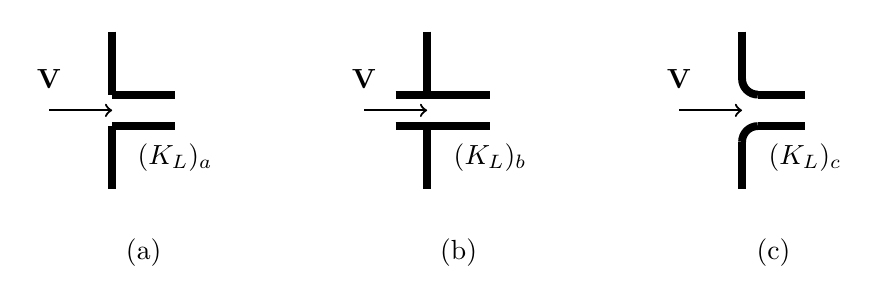
\begin{tikzpicture}[thick, scale=0.8]
\tikzstyle{beam} = [line width=1mm]
\tikzstyle{arrow} = [->, thick]
\draw[beam] (0,-1) -- (1,-1); 
\draw[beam] (0,0) -- (0,-1); 
\node at (-1, -0.75) {$\mathbf{V}$};
\draw[arrow] (-1, -1.25) -- (0, -1.25);
\draw[beam] (0, -1.5) -- (1, -1.5); 
\draw[beam] (0, -1.5) -- (0, -2.5);
\node at (1,-2) {$(K_L)_a$};

\draw[beam] (4.5,-1) -- (6,-1); 
\draw[beam] (5,0) -- (5,-1);
\node at (4, -0.75) {$\mathbf{V}$};
\draw[arrow] (4, -1.25) -- (5, -1.25);
\draw[beam] (4.5, -1.5) -- (6, -1.5);
\draw[beam] (5, -1.5) -- (5, -2.5); 
\node at (6,-2) {$(K_L)_b$};

\draw[beam] (10.25,-1) -- (11,-1); 
\draw[beam] (10,0) -- (10,-0.75); 
\node at (9, -0.75) {$\mathbf{V}$};
\draw[arrow] (9, -1.25) -- (10, -1.25);
\draw[beam] (10.25, -1.5) -- (11, -1.5); 
\draw[beam] (10, -1.75) -- (10, -2.5);
\node at (11,-2) {$(K_L)_c$};
\draw[line width=1mm] (10,-1.75) arc[start angle=180, end angle=90, radius=0.25];
\draw [line width=1mm] (10,-0.75) arc[start angle=180, end angle=270, radius=0.25];

\node at (0.5, -3.5) {(a)};
\node at (5.5, -3.5) {(b)};
\node at (10.5, -3.5) {(c)};

\end{tikzpicture}

